\chapter{Adsorption Reaction}\label{ch:adsorption}

This chapter applies the inference framework to a reaction involving
adsorption of the electroactive species onto the electrode surface.
Where \cref{ch:heterogeneous} treated an irreversible surface step
without explicit surface concentrations, the adsorption model
introduces surface coverage variables governed by ordinary differential
equations coupled to the diffusion PDE through the boundary conditions.
The Langmuir adsorption terms contain products of surface coverages and
surface concentrations, making the discrete system nonlinear and
preventing a direct banded solve. We compare three discretisation
strategies -- Newton--Raphson, explicit linearisation, and backward
implicit linearisation. Such systems arise experimentally when an
electrode is modified with a redox-active film (for example, a
  self-assembled monolayer of ferrocene-terminated thiols on
gold~\cite{compton2014understanding}) and the
voltammetry is performed in a blank electrolyte. The parameter space
grows to nine dimensions, completing the sequence $3 \to 7 \to 9$ that
structures the NUTS--RWMH comparison.

\section{Reaction Scheme}\label{sec:ads-scheme}

We consider a single electron transfer in which both the reactant
$\mathrm{A}$ and the product $\mathrm{B}$ can adsorb on the electrode
surface \cite{compton2014understanding}:
\begin{equation}\label{eq:ads-scheme}
  \mathrm{A} + \mathrm{e}^{-} \rightleftharpoons \mathrm{B}.
\end{equation}
The electron transfer can proceed through both the solution-phase
species (with rate constants $k_{\mathrm{red/ox}}^{\mathrm{sol}}$) and
the surface-bound species (with rate constants
$k_{\mathrm{red/ox}}^{\mathrm{ads}}$). Each species adsorbs onto and
desorbs from the electrode surface with rate constants
$k_{\mathrm{ads}}^{j}$ and $k_{\mathrm{des}}^{j}$, competing for a
finite number of surface sites characterised by the maximum surface
concentration $\Gamma_{\mathrm{max}}$ (\cref{fig:ads-schematic}).

\begin{figure}
  \centering
  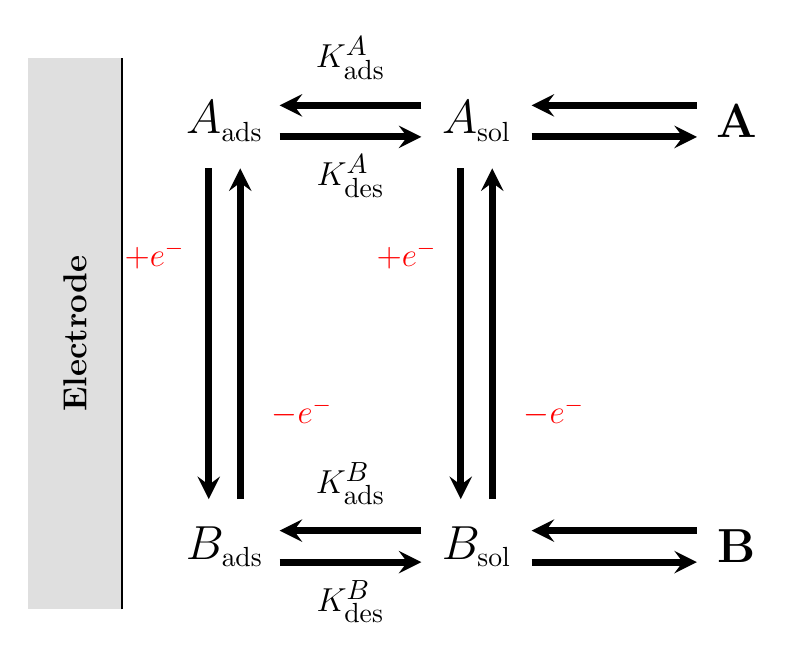
\begin{tikzpicture}[>=stealth, thick]
  % Electrode block
  \fill[gray!25] (-1.2, -1) rectangle (0, 6);
  \draw[thick] (0, -1) -- (0, 6);
  \node[rotate=90, font=\large\bfseries] at (-0.6, 2.5) {Electrode};

  % Species A row (top)
  \node[font=\LARGE\bfseries] at (1.3, 5.2) {$A_{\scriptscriptstyle
  \mathrm{ads}}$};
  \node[font=\LARGE\bfseries] at (4.5, 5.2) {$A_{\scriptscriptstyle
  \mathrm{sol}}$};
  \node[font=\LARGE\bfseries] at (7.8, 5.2) {A};

  % A: arrows
  \draw[->, line width=2.5pt] (7.3, 5.4) -- (5.2, 5.4);
  \draw[->, line width=2.5pt] (3.8, 5.4) -- (2.0, 5.4);
  \node[font=\LARGE\bfseries] at (2.9, 6.0) {$\scriptstyle K_{\scriptscriptstyle
  \mathrm{ads}}^{A}$};

  \draw[->, line width=2.5pt] (2.0, 5.0) -- (3.8, 5.0);
  \draw[->, line width=2.5pt] (5.2, 5.0) -- (7.3, 5.0);
  \node[font=\LARGE\bfseries] at (2.9, 4.5) {$\scriptstyle K_{\scriptscriptstyle
  \mathrm{des}}^{A}$};

  % Species B row (bottom)
  \node[font=\LARGE\bfseries] at (1.3, -0.2) {$B_{\scriptscriptstyle
  \mathrm{ads}}$};
  \node[font=\LARGE\bfseries] at (4.5, -0.2) {$B_{\scriptscriptstyle
  \mathrm{sol}}$};
  \node[font=\LARGE\bfseries] at (7.8, -0.2) {B};

  % B: arrows
  \draw[->, line width=2.5pt] (7.3, 0.0) -- (5.2, 0.0);
  \draw[->, line width=2.5pt] (3.8, 0.0) -- (2.0, 0.0);
  \node[font=\LARGE\bfseries] at (2.9, 0.6) {$\scriptstyle K_{\scriptscriptstyle
  \mathrm{ads}}^{B}$};

  \draw[->, line width=2.5pt] (2.0, -0.4) -- (3.8, -0.4);
  \draw[->, line width=2.5pt] (5.2, -0.4) -- (7.3, -0.4);

  \node[font=\LARGE\bfseries] at (2.9, -0.9) {$\scriptstyle
    K_{\scriptscriptstyle
  \mathrm{des}}^{B}$};

  % Electron solution transfer arrows
  \draw[->, line width=2.5pt] (4.3, 4.6) -- (4.3, 0.4);
  \node[left, font=\large] at (6.0, 1.5) {\textcolor{red}{$-e^-$}};
  \draw[->, line width=2.5pt] (4.7, 0.4) -- (4.7, 4.6);
  \node[right, font=\large] at (3.1, 3.5) {\textcolor{red}{$+e^-$}};

  % Electron adsorption transfer arrows
  \draw[->, line width=2.5pt] (1.1, 4.6) -- (1.1, 0.4);
  \node[left, font=\large] at (2.8, 1.5) {\textcolor{red}{$-e^-$}};
  \draw[->, line width=2.5pt] (1.5, 0.4) -- (1.5, 4.6);
  \node[right, font=\large] at (-0.1, 3.5) {\textcolor{red}{$+e^-$}};

\end{tikzpicture}

  \caption[Schematic of the adsorption reaction]{Schematic of the
    adsorption reaction mechanism. Species $\mathrm{A}$ and $\mathrm{B}$
    exist in both a solution phase and a surface-bound (adsorbed) phase.
    Electron transfer can occur between both solution-phase and
    adsorbed species. Adsorption and desorption exchange species between
  the two phases.}
  \label{fig:ads-schematic}
\end{figure}

The solution-phase and adsorbed electron transfers are each
characterised by their own transfer coefficient and rate constant:
$(\alpha^{\mathrm{sol}},\, K_0^{\mathrm{sol}})$ and
$(\alpha^{\mathrm{ads}},\, K_0^{\mathrm{ads}})$ respectively. The nine
parameters to be inferred are
\begin{equation}\label{eq:ads-params}
  \phi = \bigl(\alpha^{\mathrm{sol}},\, K_0^{\mathrm{sol}},\,
    \theta_f^{\mathrm{sol}},\,
    \alpha^{\mathrm{ads}},\, K_0^{\mathrm{ads}},\,
    K_{\mathrm{ads}}^{\mathrm{A}},\, K_{\mathrm{des}}^{\mathrm{A}},\,
    K_{\mathrm{ads}}^{\mathrm{B}},\, K_{\mathrm{des}}^{\mathrm{B}}
  \bigr) \in \mathbb{R}^9.
\end{equation}
The saturation parameter $\beta = c_\mathrm{A}^*\,r_e/
\Gamma_{\mathrm{max}}$ is treated as known and fixed at $\beta = 1$.

\section{Mathematical Description}\label{sec:ads-maths}

\subsection{Governing Equations}

The transport of $\mathrm{A}$ and $\mathrm{B}$ in solution is governed
by the same dimensionless diffusion equation as in
\cref{eq:nd_diffusion}:
\begin{equation}\label{eq:ads-diffusion}
  \frac{\partial C_j}{\partial T} = \frac{\partial^2 C_j}{\partial X^2},
  \qquad j \in \{\mathrm{A},\,\mathrm{B}\}.
\end{equation}
Unlike the heterogeneous reaction of \cref{ch:heterogeneous}, there are
no kinetic source terms in the bulk. All coupling between the species
enters through the boundary conditions at the electrode surface.

\subsection{Surface Coverage Equations}

The surface coverages $\xi_j = \Gamma_j / \Gamma_{\mathrm{max}}$
evolve according to
\begin{equation}\label{eq:ads-coverage-ode}
  \begin{aligned}
    \frac{\mathrm{d}\xi_\mathrm{A}}{\mathrm{d}T}
    &= -K_{\mathrm{red}}^{\mathrm{ads}}\,\xi_\mathrm{A}
    + K_{\mathrm{ox}}^{\mathrm{ads}}\,\xi_\mathrm{B}
    + K_{\mathrm{ads}}^{\mathrm{A}}\,C_{0,\mathrm{A}}
    \bigl[1 - (\xi_\mathrm{A} + \xi_\mathrm{B})\bigr]
    - K_{\mathrm{des}}^{\mathrm{A}}\,\xi_\mathrm{A}, \\[4pt]
    \frac{\mathrm{d}\xi_\mathrm{B}}{\mathrm{d}T}
    &= K_{\mathrm{red}}^{\mathrm{ads}}\,\xi_\mathrm{A}
    - K_{\mathrm{ox}}^{\mathrm{ads}}\,\xi_\mathrm{B}
    + K_{\mathrm{ads}}^{\mathrm{B}}\,C_{0,\mathrm{B}}
    \bigl[1 - (\xi_\mathrm{A} + \xi_\mathrm{B})\bigr]
    - K_{\mathrm{des}}^{\mathrm{B}}\,\xi_\mathrm{B},
  \end{aligned}
\end{equation}
where $C_{0,j} = C_j(T, 0)$ is the surface concentration in solution.
The first two terms in each equation are the adsorbed electron transfer;
the third is Langmuir adsorption, with $[1 - (\xi_\mathrm{A} +
\xi_\mathrm{B})]$ the fraction of unoccupied sites; the fourth is
desorption.

\subsection{Electrode Boundary Conditions}

The surface flux of each species is determined by the solution-phase
electron transfer and the net adsorption/desorption flux:
\begin{equation}\label{eq:ads-bc}
  \begin{aligned}
    \left(\frac{\partial C_\mathrm{A}}{\partial X}\right)_{X=0}
    &= K_{\mathrm{red}}^{\mathrm{sol}}\,C_{0,\mathrm{A}}
    - K_{\mathrm{ox}}^{\mathrm{sol}}\,C_{0,\mathrm{B}}
    + K_{\mathrm{ads}}^{\mathrm{A}}\,C_{0,\mathrm{A}}
    \bigl[1 - (\xi_\mathrm{A} + \xi_\mathrm{B})\bigr]
    - K_{\mathrm{des}}^{\mathrm{A}}\,\xi_\mathrm{A}, \\[4pt]
    \left(\frac{\partial C_\mathrm{B}}{\partial X}\right)_{X=0}
    &= \frac{1}{d_\mathrm{B}}\Bigl\{
      -K_{\mathrm{red}}^{\mathrm{sol}}\,C_{0,\mathrm{A}}
      + K_{\mathrm{ox}}^{\mathrm{sol}}\,C_{0,\mathrm{B}}
      + K_{\mathrm{ads}}^{\mathrm{B}}\,C_{0,\mathrm{B}}
      \bigl[1 - (\xi_\mathrm{A} + \xi_\mathrm{B})\bigr]
      - K_{\mathrm{des}}^{\mathrm{B}}\,\xi_\mathrm{B}
    \Bigr\}.
  \end{aligned}
\end{equation}
The dimensionless rate constants follow the Butler--Volmer form:
\begin{equation}\label{eq:ads-kred-kox}
  \begin{aligned}
    K_{\mathrm{red}}^{\mathrm{sol}}
    &= K_0^{\mathrm{sol}}
    \exp\!\bigl[-\alpha^{\mathrm{sol}}\bigl(\theta(T) -
    \theta_f^{\mathrm{sol}}\bigr)\bigr],
    &\qquad
    K_{\mathrm{ox}}^{\mathrm{sol}}
    &= K_0^{\mathrm{sol}}
    \exp\!\bigl[(1-\alpha^{\mathrm{sol}})\bigl(\theta(T) -
    \theta_f^{\mathrm{sol}}\bigr)\bigr],
    \\[4pt]
    K_{\mathrm{red}}^{\mathrm{ads}}
    &= K_0^{\mathrm{ads}}
    \exp\!\bigl[-\alpha^{\mathrm{ads}}\bigl(\theta(T) -
    \theta_f^{\mathrm{ads}}\bigr)\bigr],
    &\qquad
    K_{\mathrm{ox}}^{\mathrm{ads}}
    &= K_0^{\mathrm{ads}}
    \exp\!\bigl[(1-\alpha^{\mathrm{ads}})\bigl(\theta(T) -
    \theta_f^{\mathrm{ads}}\bigr)\bigr],
  \end{aligned}
\end{equation}
where $K_0^{\mathrm{sol}} = k_0^{\mathrm{sol}}\,r_e/ D_\mathrm{A}$
and $K_0^{\mathrm{ads}} = k_0^{\mathrm{ads}}\,r_e^2 / D_\mathrm{A}$.
The formal potentials of the two couples are related by thermodynamic
consistency \cite{compton2014understanding}:
\begin{equation}\label{eq:ads-thetaf-relation}
  \theta_f^{\mathrm{ads}} = \theta_f^{\mathrm{sol}}
  - \ln\!\left(
    \frac{K_{\mathrm{ads}}^{\mathrm{A}} / K_{\mathrm{des}}^{\mathrm{A}}}
    {K_{\mathrm{ads}}^{\mathrm{B}} / K_{\mathrm{des}}^{\mathrm{B}}}
  \right).
\end{equation}
This is not an additional free parameter: $\theta_f^{\mathrm{ads}}$ is
determined by $\theta_f^{\mathrm{sol}}$ and the four
adsorption/desorption dimensionless rate constants already in~$\phi$
which are of the form
\begin{equation}\label{eq:ads-kads-kdes}
  K_{\mathrm{ads}}^{j}
  = \frac{k_{\mathrm{ads}}^{j}\,\Gamma_{\mathrm{max}}\,r_e}
  {D_\mathrm{A}},
  \qquad
  K_{\mathrm{des}}^{j}
  = \frac{k_{\mathrm{des}}^{j}\,\Gamma_{\mathrm{max}}\,r_e}
  {c_\mathrm{A}^*\,D_\mathrm{A}}.
\end{equation}

\subsection{Initial Conditions}

Initially only species $\mathrm{A}$ is present in solution at its bulk
concentration: $C_\mathrm{A}(0, X) = 1$, $C_\mathrm{B}(0, X) = 0$.
The initial surface coverages are set by the Langmuir equilibrium:
\begin{equation}\label{eq:ads-ic-coverage}
  \xi_\mathrm{A}(0) =
  \frac{K_{\mathrm{ads}}^{\mathrm{A}} / K_{\mathrm{des}}^{\mathrm{A}}}
  {1 + K_{\mathrm{ads}}^{\mathrm{A}} / K_{\mathrm{des}}^{\mathrm{A}}
    + C_\mathrm{B}^*\, K_{\mathrm{ads}}^{\mathrm{B}} /
  K_{\mathrm{des}}^{\mathrm{B}}},
  \qquad
  \xi_\mathrm{B}(0) =
  \frac{C_\mathrm{B}^*\, K_{\mathrm{ads}}^{\mathrm{B}} /
  K_{\mathrm{des}}^{\mathrm{B}}}
  {1 + K_{\mathrm{ads}}^{\mathrm{A}} / K_{\mathrm{des}}^{\mathrm{A}}
    + C_\mathrm{B}^*\, K_{\mathrm{ads}}^{\mathrm{B}} /
  K_{\mathrm{des}}^{\mathrm{B}}}.
\end{equation}

We set $C_\mathrm{B}^* = 0$ and thus $\xi_\mathrm{B}(0) = 0$.

\subsection{Current}

The measured current has contributions from both the solution-phase and
adsorbed electron transfers:
\begin{equation}\label{eq:ads-current}
  \frac{I}{\pi r_e F D_\mathrm{A} c_\mathrm{A}^*}
  = -\left\{
    \left(\frac{\partial C_\mathrm{A}}{\partial X}\right)_{X=0}
    - \frac{1}{\beta}
    \frac{\mathrm{d}\xi_\mathrm{A}}{\mathrm{d}T}
  \right\}.
\end{equation}
The first term is the diffusive flux; the second accounts for charge
transferred by the conversion of adsorbed $\mathrm{A}$ to adsorbed
$\mathrm{B}$.

\section{Nonlinearity and Discretisation}\label{sec:ads-disc}

The Langmuir terms in \cref{eq:ads-coverage-ode,eq:ads-bc} contain
products of the unknown surface concentrations $C_{0,j}$ and surface
coverages $\xi_j$ at the current timestep. After backward Euler
discretisation these become products of unknowns at timestep~$k$,
making the algebraic system nonlinear -- in contrast to
\cref{ch:heterogeneous}, where all coupling was linear and the system
could be solved directly.

\subsection{Newton--Raphson Solver}\label{sec:ads-newton}

We order the unknowns as $\mathbf{x} = (\xi_\mathrm{A}^k,\,
  \xi_\mathrm{B}^k,\, C_{0,\mathrm{A}}^k,\, C_{0,\mathrm{B}}^k,\,
\ldots,\, C_{n-1,\mathrm{A}}^k,\, C_{n-1,\mathrm{B}}^k)^T$ and solve
the nonlinear residual $\mathbf{F}(\mathbf{x}) = 0$ by Newton--Raphson
iteration, using the previous timestep's solution as the initial guess.
After a preliminary row elimination to decouple the surface coverage
from the far-field equations~\cite{compton2014understanding}, the
Jacobian reduces to pentadiagonal form. We solve to tight tolerances
($r_{\mathrm{tol}} = 10^{-10}$, $a_{\mathrm{tol}} = 10^{-12}$) so
that this solver serves as the ground-truth reference. One could fix
the iteration count to make the solver traceable by reverse-mode AD,
but this neither guarantees convergence nor avoids the cost of
differentiating through every Newton step. We therefore require a
linearised alternative for inference.

\subsection{Alternative Solvers}\label{sec:ads-alt-solvers}

Two strategies linearise the nonlinear terms at each timestep, producing
systems solvable directly and differentiable through.

\paragraph{Explicit linearisation.}
The products $C_{0,j}^k\,[1 - (\xi_\mathrm{A}^k +
\xi_\mathrm{B}^k)]$ are approximated by evaluating the surface
coverage at the previous timestep:
\begin{equation}\label{eq:ads-explicit}
  C_{0,j}^k\,\bigl[1 - (\xi_\mathrm{A}^k + \xi_\mathrm{B}^k)\bigr]
  \approx
  C_{0,j}^k\,\bigl[1 - (\xi_\mathrm{A}^{k-1} + \xi_\mathrm{B}^{k-1})\bigr].
\end{equation}
This is first-order in $\Delta T$ and accurate when the surface
coverage does not change rapidly between timesteps.

Following Britz~\cite{britz2016digital}, the product is expanded to
first order about the previous-timestep values:
\begin{equation}\label{eq:ads-britz}
  C_{0,j}^k\,\xi_l^k
  \approx
  C_{0,j}^k\,\xi_l^{k-1}
  + C_{0,j}^{k-1}\,\xi_l^k
  - C_{0,j}^{k-1}\,\xi_l^{k-1}.
\end{equation}
This retains linear coupling to both unknowns at timestep~$k$, also
first-order in $\Delta T$ but with more implicit coupling than the
explicit scheme. Both alternatives produce a pentadiagonal system after
row elimination which is compatible with the adjoint framework of
\cref{ch:adjoint}.

\subsection{Solver Comparison}\label{sec:ads-solver-comparison}

\Cref{fig:ads-solver-comparison} compares the two AD-compatible solvers
against the Newton reference. The backward implicit scheme achieves
errors of order $10^{-7}$ across most of the sweep, compared with
$10^{-3}$ for the explicit scheme. For both solvers, the error
increases when we have a fast change in the gradient of the current.

\begin{figure}[ht]
  \centering
  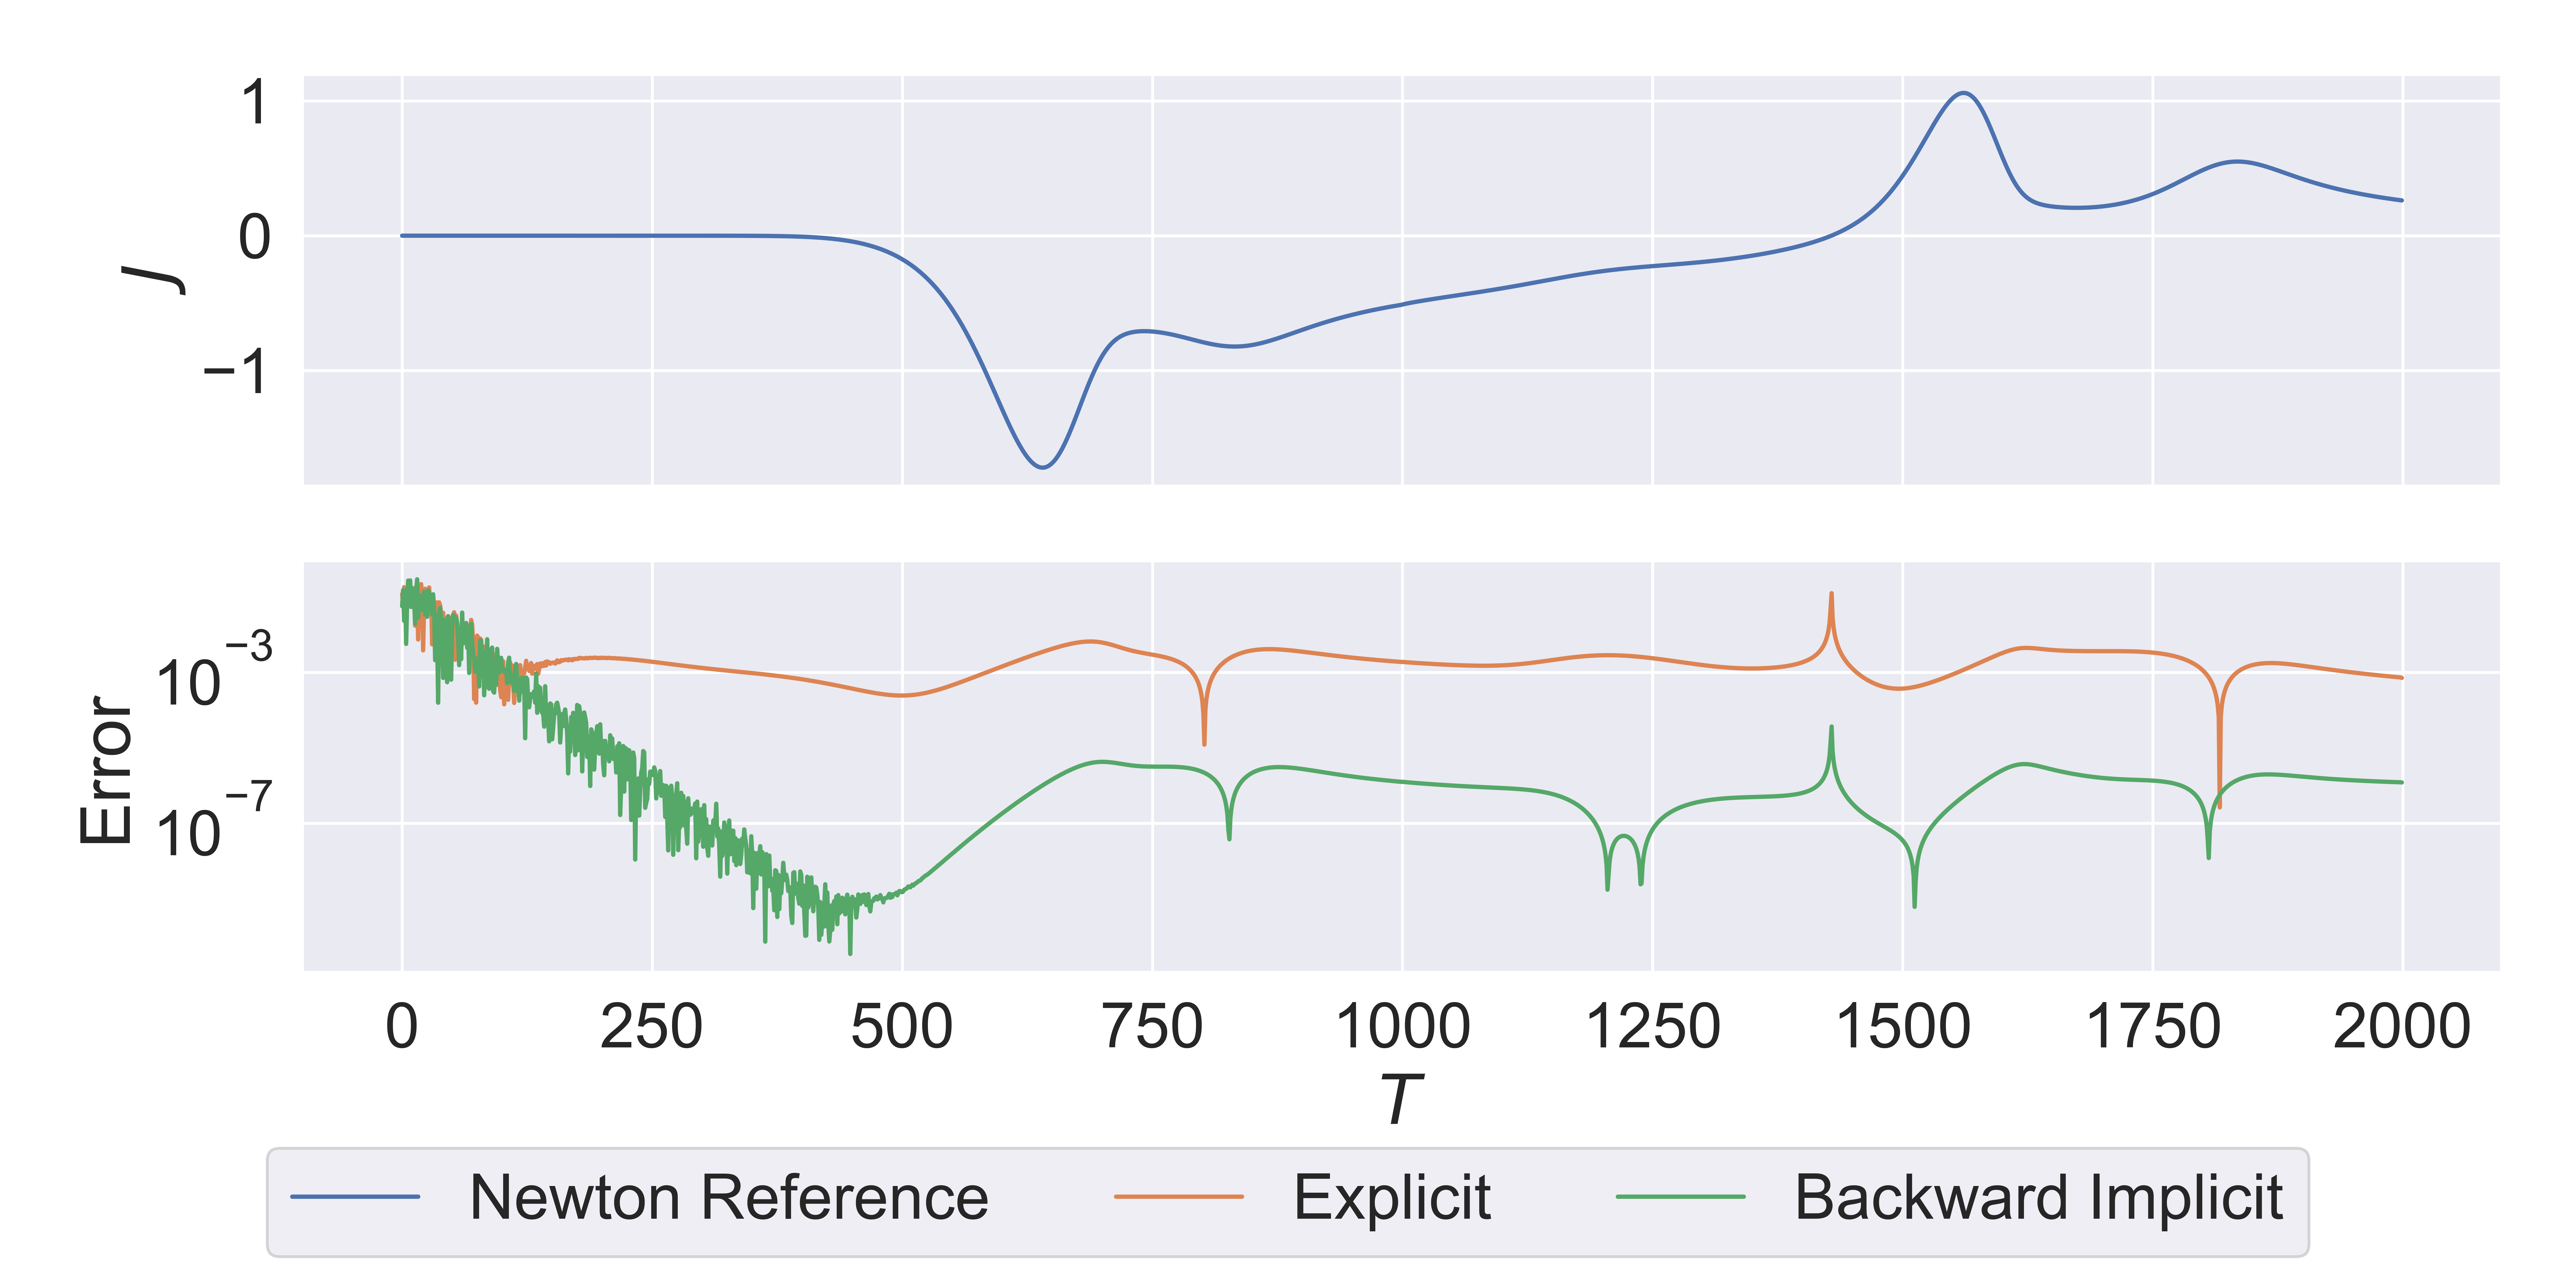
\includegraphics[width=0.95\textwidth]{figures/8-solver-comparison.png}
  \caption[Solver comparison for the adsorption reaction]{Top:
    Reference Newton current against time. Bottom: Absolute
    relative error of the explicit (orange) and backward implicit (green)
    solvers against the Newton reference at each timestep. The backward
    implicit scheme is three to four orders of magnitude more accurate
  across most of the sweep.}
  \label{fig:ads-solver-comparison}
\end{figure}

The backward implicit solver is slower than the explicit solver
(80\,ms vs 60\,ms per forward solve). This 33\% overhead is
acceptable given the accuracy gain, and we adopt the backward implicit
scheme for all inference runs.

\section{Inference Setup}\label{sec:ads-inference}

The inference workflow follows \cref{sec:workflow} without modification.
The transfer coefficients are logit-transformed, the rate constants
log-transformed, and $\theta_f^{\mathrm{sol}}$ left untransformed.
Synthetic data are generated using the Newton solver at the true
parameter values
\begin{equation}\label{eq:ads-true-params}
  \phi^* = (0.5,\; 10^{-3},\; 0.0,\; 0.45,\; 0.5,\;
  4.5,\; 1.0,\; 1.0,\; 1.0),
\end{equation}
with dimensionless scan rate $\sigma = 10$ and noise level
$\eta = 0.02$. The scan rate is two orders of magnitude lower than the
$\sigma = 1000$ used in the preceding chapters: adsorption and
desorption operate on a slower timescale than electron transfer, and at
high scan rates the potential sweeps too fast for adsorption to respond,
rendering the voltammogram insensitive to the adsorption rate constants.

\section{Results}\label{sec:ads-results}

\subsection{Solver Verification}\label{sec:ads-verification}

We verify the forward solver against the analytical solution for a pure
monolayer -- a system in which all electroactive material is
pre-adsorbed and no solution-phase electron transfer occurs. For a
fully reversible adsorbed redox couple the dimensionless current is
\cite{chen2026differentiable}
\begin{equation}\label{eq:ads-monolayer-analytical}
  J = \mp\,\frac{\exp(-\theta)}{(1 + \exp(-\theta))^2},
\end{equation}
where the upper sign refers to the cathodic scan and the lower to the
anodic scan. \Cref{fig:ads-verification} confirms that the numerical
solution reproduces the full analytical trajectory.

\begin{figure}[ht]
  \centering
  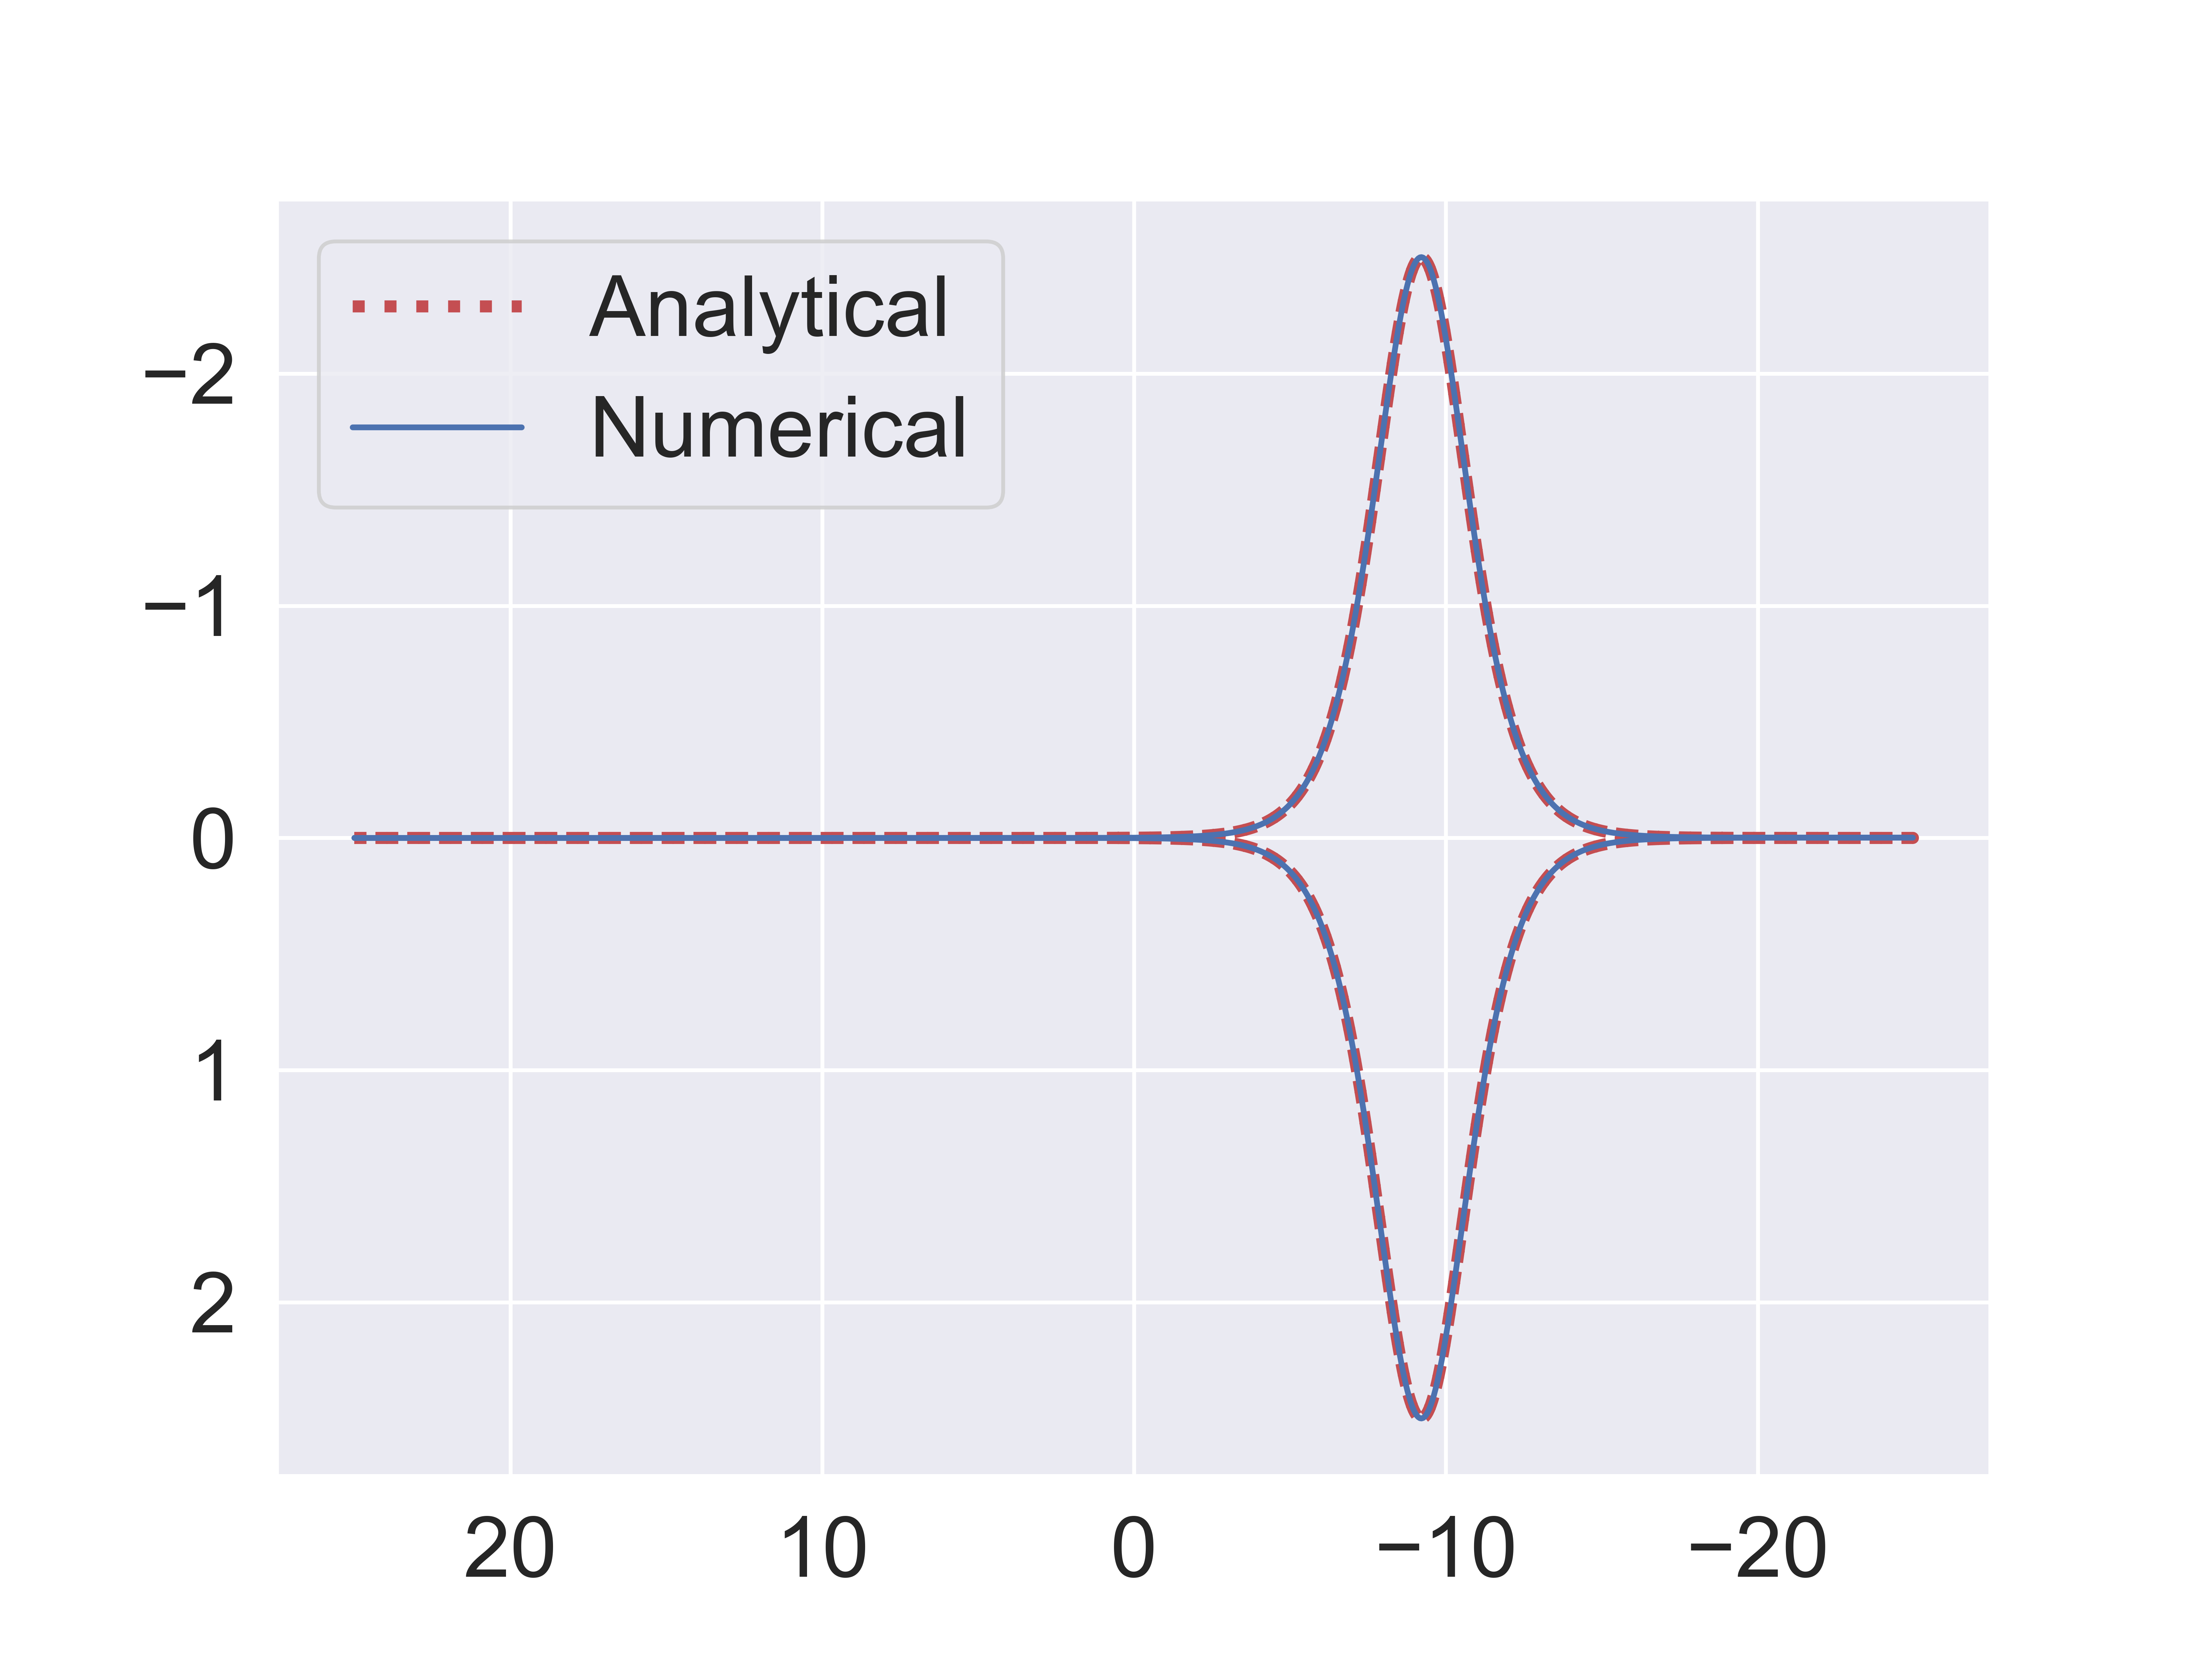
\includegraphics[width=0.5\textwidth]{figures/8-analytical.png}
  \caption[Verification against the monolayer analytical
  solution]{Voltammogram for a pure monolayer with a reversible adsorbed
    redox couple. The numerical solution (solid) matches the analytical
  current~\cref{eq:ads-monolayer-analytical} (dashed).}
  \label{fig:ads-verification}
\end{figure}

\subsection{Posterior Distributions}\label{sec:ads-posteriors}

\Cref{fig:ads-corner} shows pairwise marginal posteriors from NUTS
(2\,800 samples) and RWMH (40\,000 samples) under equal computational
budgets. Both samplers recover the true parameter values.
$\theta_f^{\mathrm{sol}}$ omitted for brevity.

The off-diagonal panels reveal the correlation structure.
$\alpha^{\mathrm{sol}}$ and $K_0^{\mathrm{sol}}$ are correlated due to
the kinetic trade-off in the Butler--Volmer equation, as in the
lower-dimensional cases; the same holds for $\alpha^{\mathrm{ads}}$ and
$K_0^{\mathrm{ads}}$. The adsorption and desorption rate constants for
each species are also correlated: the Langmuir terms
in~\cref{eq:ads-coverage-ode,eq:ads-bc} depend on these constants
primarily through the equilibrium ratio
$K_{\mathrm{ads}}^{j}/K_{\mathrm{des}}^{j}$, which sets the surface
coverage at steady state. Increasing both constants by the same factor
leaves this ratio nearly unchanged, producing a similar voltammogram.
The posterior is therefore elongated along the direction in which the
ratio is constant -- visible in the corner plot as diagonal contours
in the $K_{\mathrm{ads}}^{j}$ vs $K_{\mathrm{des}}^{j}$ panels. This
geometry makes sampling harder: moving along the ridge is easy, but
resolving the narrow cross-section requires precise steps, reducing
efficiency for both samplers as we quantify in \cref{sec:ads-ess}.
Despite these correlations, both samplers resolve the individual rate
constants.

\begin{figure}[ht]
  \centering
  \includegraphics[width=1.00\textwidth]{figures/8-corner.png}
  \caption[Pairwise posteriors for the adsorption
  reaction]{Pairwise marginal posteriors for the adsorption
    reaction. NUTS (blue) and RWMH (orange) are overlaid; dashed lines
    indicate the true parameter values. $\theta_f^{\mathrm{sol}}$
  omitted for brevity}
  \label{fig:ads-corner}
\end{figure}

That both samplers recover the true parameters -- despite inference
using the backward implicit linearisation rather than the Newton solver
that generated the data -- confirms that the
approximation~\cref{eq:ads-britz} does not introduce systematic bias at
this noise level.

\Cref{fig:ads-current-fit} overlays the posterior-mean voltammogram
with the true current. The 95\% credible interval is tight throughout
the sweep.

\begin{figure}[ht]
  \centering
  \includegraphics[width=0.7\textwidth]{figures/8-current-fit.png}
  \caption[Current fit for the adsorption reaction]{Posterior-mean
    voltammogram (solid) with 95\% credible interval (shaded) against
  the true current (dashed) and noisy data (points).}
  \label{fig:ads-current-fit}
\end{figure}

\subsection{Sampling Efficiency}\label{sec:ads-ess}

\Cref{fig:ads-ess} compares ESS growth for NUTS and RWMH on a
normalised cost axis. \Cref{tab:ads-ess} reports the final values with
NUTS/RWMH ratios. The results split into two groups. For the
solution-phase and adsorbed electron-transfer parameters
($\alpha^{\mathrm{sol}}$, $K_0^{\mathrm{sol}}$,
  $\theta_f^{\mathrm{sol}}$, $\alpha^{\mathrm{ads}}$,
$K_0^{\mathrm{ads}}$), the ratios are $4.0$--$4.8\times$, continuing
the upward trend from $1.5$--$2.4\times$ in three dimensions
(\cref{sec:hmc-results}) and $2.7$--$3.6\times$ in seven
(\cref{sec:het-ess}). For the adsorption/desorption rate constants the
ratios are lower, $2.3$--$2.6\times$: the elongated posterior geometry
described in \cref{sec:ads-posteriors} reduces the advantage of
gradient-based proposals, since both samplers struggle to resolve the
narrow cross-section of the ridge.

\begin{table}[ht]
  \centering
  \begin{tabular}{lccccccccc}
    \hline
    & $\alpha^{\mathrm{sol}}$ & $K_0^{\mathrm{sol}}$ & $\theta_f^{\mathrm{sol}}$
    & $\alpha^{\mathrm{ads}}$ & $K_0^{\mathrm{ads}}$
    & $K_{\mathrm{ads}}^{\mathrm{A}}$
    & $K_{\mathrm{des}}^{\mathrm{A}}$
    & $K_{\mathrm{ads}}^{\mathrm{B}}$
    & $K_{\mathrm{des}}^{\mathrm{B}}$ \\
    \hline
    NUTS & 4860.8 & 5527.5 & 4402.0 & 4707.2 & 5334.7 & 3451.7 &
    3319.6 & 3807.2 & 3501.9
    \\
    RWMH & 1185.0 & 1139.9 & 1113.7 & 1160.2 & 1311.9 & 1484.3 &
    1405.7 & 1439.8 & 1493.0
    \\
    Ratio & 4.1 & 4.8 & 4.0 & 4.1 & 4.1 & 2.3 & 2.4 & 2.6 & 2.3 \\
    \\
    \hline
  \end{tabular}
  \caption[ESS for the adsorption reaction]{Effective sample size for
    each parameter for 40\,000 RWMH samples and 2\,800 NUTS samples at
  equal sampling runtime, with NUTS/RWMH ratio.}
  \label{tab:ads-ess}
\end{table}

\begin{figure}[ht]
  \centering
  \includegraphics[width=0.95\textwidth]{figures/8-ess.png}
  \caption[ESS comparison for the adsorption reaction]{Effective
    sample size as a function of sample proportion for each parameter.
    NUTS (blue) accumulates independent samples at a higher rate than
  RWMH (orange) across all nine parameters.}
  \label{fig:ads-ess}
\end{figure}
